\section{“麻雀“OS--uCore}

为了学习OS,需要了解一个上百万代码的操作系统吗?自己写一个操作系统难吗?别被现在上百万行的Linux和Windows操作系统吓倒。当年Thompson乘他老婆带着小孩度假留他一人在家时,写了UNIX;当年Linus还是一个21岁大学生时完成了Linux雏形。站在这些巨人的肩膀上,我们能否也尝试一下做“巨人”的滋味呢?

MIT的Frans Kaashoek等在2006年参考PDP-11上的UNIX Version 6写了一个可在X86上跑的操作系统xv6(基于MIT License),用于学生学习操作系统。我们可以站在他们的肩膀上,基于xv6的设计,尝试着一步一步完成一个从“空空如也”到“五脏俱全”的“麻雀”操作系统—ucore,此“麻雀”包含虚存管理、进程管理、处理器调度、同步互斥、进程间通信、文件系统等主要内核功能,总的内核代码量(C+asm)不会超过5K行。充分体现了“小而全”的指导思想。

ucore的运行环境可以是真实的计算机系统,目前支持运行在X86,MIPS,ARM,RISC-V等计算机系统中。不过考虑到调试和开发的方便,我们可采用硬件模拟器,比如QEMU、BOCHS、VirtualBox、VMware Player等。ucore的开发环境主要是GCC中的gcc、gas、ld和MAKE等工具,也可采用集成了这些工具的IDE开发环境Eclipse-CDT。运行环境和开发环境既可以在Linux或Windows中使用。

那我们准备如何一步一步实现ucore呢?安装一个操作系统的开发过程,我们可以有如下的开发步骤:

\begin{enumerate}
	\def\labelenumi{\arabic{enumi}.}
	\item
	bootloader+toy
	ucore:理解操作系统启动前的硬件状态和要做的准备工作,了解运行操作系统的外设硬件支持,操作系统如何加载到内存中,理解两类中断--``外设中断'',``陷阱中断'',内核态和用户态的区别;
	\item
	物理内存管理:理解x86分段/分页模式,了解操作系统如何管理物理内存;
	\item
	虚拟内存管理:理解OS虚存的基本原理和目标,以及如何结合页表+中断处理(缺页故障处理)来实现虚存的目标,如何实现基于页的内存替换算法和替换过程;
	\item
	内核线程管理:理解内核线程创建、执行、切换和结束的动态管理过程,以及内核线程的运行周期等;
	\item
	用户进程管理:理解用户进程创建、执行、切换和结束的动态管理过程,以及在用户态通过系统调用得到内核中各种服务的过程;
	\item
	处理器调度:理解操作系统的调度过程和调度算法;
	\item
	同步互斥与进程间通信:理解同步互斥的具体实现以及对系统性能的影响,研究死锁产生的原因,如何避免死锁,以及线程/进程间如何进行信息交换和共享;
	\item
	文件系统:理解文件系统的具体实现,与进程管理和内存管理等的关系,缓存对操作系统IO访问的性能改进,虚拟文件系统(VFS)、buffer~cache和disk~driver之间的关系。
\end{enumerate}

其中每个开发步骤都是建立在上一个步骤之上的,就像搭积木,从一个一个小木块,最终搭出来一个小房子。在搭房子的过程中,完成从理解操作系统原理到实践操作系统设计与实现的探索过程。

%这个房子最终的建筑架构和建设进度如下图所示
%\textgreater{} (!可进一步标注处各个proj在下图中的位置)
%\begin{figure}[htbp]
%	\centering
%	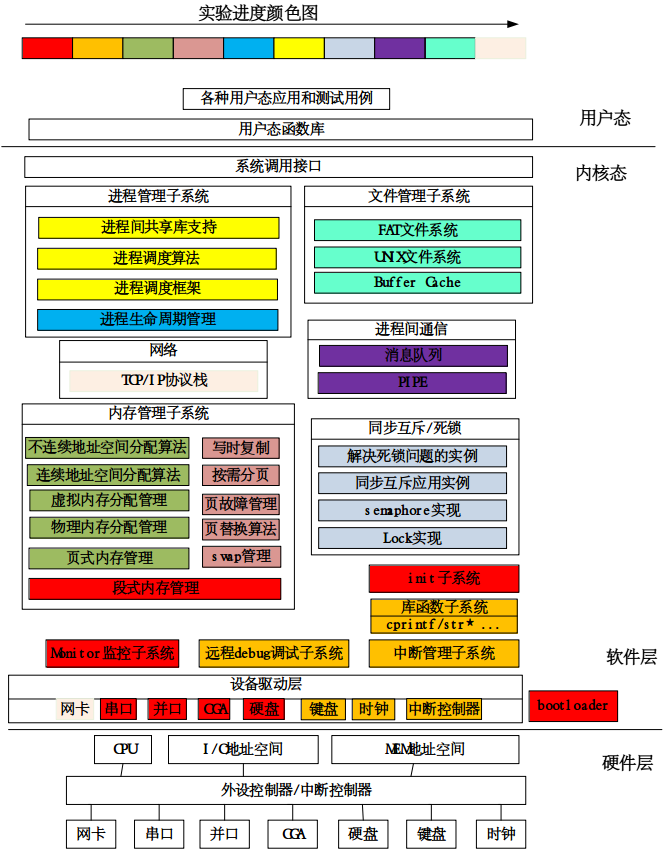
\includegraphics{figures/ucore_arch.png}
%	\caption{ucore操作系统架构}
%\end{figure}